%\documentclass[12pt]{memoir}
\documentclass[12pt]{workjournal}


\author{Joe Schoonover \\ Dhruv Balwada}
\date{}




\begin{document}


\frontmatter

%%%%%%%%%%%%%%%%%%%%%%%%%%%%%%%%%%%%%%%%%%%%%%%%%%%%%%%%%%%%%%%%%
% Custom Title Page 
%%%%%%%%%%%%%%%%%%%%%%%%%%%%%%%%%%%%%%%%%%%%%%%%%%%%%%%%%%%%%%%%%
\begin{titlingpage}
    
        \vspace*{2cm}

   % Setup up the main and sub-titles with the logo
   {\fontfamily{cmss}\selectfont
     \begin{tabular}{l r}
           & \HUGE{\textbf{ Balanced Flow Topographic Interactions }}\\

        \end{tabular}
    }    
 
        \vspace{1cm}
        

         
        \vspace{2cm}
        
     \begin{center}
     
        %Do a subtitle here if you like
        {\fontfamily{cmss}\selectfont
        \huge{
           Project Plan and Theory
        }
        
        \vspace{1.5cm}
        
        % Enter the author's name
        \textbf{
        \large{
           \theauthor 
         }}}
        
        \vfill
        
        
     \end{center}
        
    
\end{titlingpage}

%%%%%%%%%%%%%%%%%%%%%%%%%%%%%%%%%%%%%%%%%%%%%%%%%%%%%%%%%%%%%%%%%
% Table of Contents and a list of modules
%%%%%%%%%%%%%%%%%%%%%%%%%%%%%%%%%%%%%%%%%%%%%%%%%%%%%%%%%%%%%%%%%

{\fontfamily{cmss}\selectfont
\tableofcontents
}
\vspace{1cm}
\hrule


% Special Style
\pagestyle{myheadings}
\mainmatter

\chapter{Motivating Questions}
\textit{with some citations and additional ``filler'' this would make a solid introduction...(Credit to Dhruv)}\\

There are two problems in the ocean that people believe are unsolved to some extent (we know everything and nothing). The first being the missing mixing: \textit{\textbf{How do dense waters formed at the poles eventually become light to maintain the current stratification of the ocean (particularly the deep ocean)?}} The second being the missing forward cascade: \textit{\textbf{How do balanced flows lose the energy that is supplied to them via winds in the face of turbulence theories predicting large scale flows to have an inverse energy cascade?}} The two problems are completely intertwined via the threads of turbulence, as dissipation and mixing \underline{almost} always go hand in hand. Different mechanisms have been proposed to answer each problem to some degree. The emerging idea is that ocean boundaries, which we barely understand, are where we will find answers to both these problems.


The questions we are interested in answering :
\begin{enumerate}
\item How do dense waters formed at the poles eventually become light to maintain the current stratification of the ocean ? Another way to say this is that we are interested in understanding better how mass balance is achieved in the thermohaline circulation - if cold water continually sinks at the poles, where does it come up and how long does it take ? To answer this, we need to understand the processes that lead to water mass transformation.
\item  Given that large scale geophysical turbulence exhibits an inverse cascade and the oceans are not continually accelerating, how does the general circulation dissipate its energy ?
\item Is topography able to catalyze the transfer of energy from large scale balanced flows to small scale unbalanced flows that inevitably lead to dissipation ?
\item Can balanced flow interactions with topography provide a means of enhancing water mass mixing ? Where would this mixing take place ?
\end{enumerate}
** A follow-up to question (3) : The development of sharp buoyancy gradients may lead to mixing of the buoyancy field which modifies the potential energy. It's not clear to me yet how this relates to the loss of total energy. Does kinetic energy get transferred to potential energy, and through mixing leads to a loss of total energy ? Is kinetic energy dissipated directly through scale transfers, bypassing the potential energy channel ? I would like to make an "energetic-transfer-map" that shows the pathway that the balanced energy takes.

\textit{At this point, I think there are plenty of questions to answer. Identifying previous work in the literature clearly is a good plan to start. I've included a .bib file with references that I feel are useful. Below, Chapter (\ref{chapter:references}) is where we can include paragraph summaries of relevant papers - I've found this to be useful when it comes time to write a paper.}


\chapter{Working plan}
 The focus of this project is primarily on the interactions of large scale balanced flows and topography. Shelf wave theory \citep{Buchwald1968,Rhines1970,Huthnance1975,Huthnance1978,Hughes1986} describes the natural wave modes that develop over variable bathymetry and in the presence of stratification. These natural modes can interact with large scale, low frequency flows such as in the case of the Gulf Stream \citep{Xue1992,Lozier2005}. Recent work involving interactions of a balanced flow with a vertical wall illustrates how the arrest of Kelvin waves (a subset of shelf waves, see \citep{ChapmanRizzoli1989} for dispersion diagram) by the balanced can lead to shock formation, small scale development, and enhanced mixing \citep{Dewar2010,Hogg2011}. Kelvin wave hydraulic control provides a mechanism that can transfer energy out of the large scale balanced flow and into small scale balanced flows.
 
\textit{\textbf{Goal 1 :}}\\ 
 \textit{ Quantification of the energy transfer rates of Kelvin Wave Hydraulic conrol will provide necessary quantitative information to determine if this mechanism is efficient enough to considerably impact global energetic balances. Additionally, determining the dynamic interchanges of kinetic and potential energy will provide useful details in describing the means by which the total energy is lost from the balanced flow.}
 
\textit{\textbf{Goal 2 :}}\\
\textit{ The extension of Kelvin wave hydraulic control to general shelf waves that are present over sloping topography is currently unclear but is the obvious next step to generalizing the theory of \citet{Hogg2011}. Whether the arrest mechanism is possible and leads to similar shock formation is still an open question. ``Long wave theory'', explored by \citep{Hughes1986,Stern1998}, allows for wave arrest to occur due to the lack of wave dispersion. Including shorter shelf wave modes leads to dispersion of shelf waves that allows for scattering of energy rather than the focusing of energy at small length scales. The details of the long and short wave behaviors need to be clarified.}
 
 \section{Towards Goal 1}
 Hydrostatic primitive simulations will be configured in a similar setup to \citep{Dewar2010} and  of the kinetic, potential, and total energies and the associated components of the total energy equation will be monitored in bulk volume integrals to determine the dynamic transition of energy between kinetic and potential energy and any dissipation. The SELF-HPE model \citep{schoonoverSEM} will be applied with an Adaptive Roll-off Filter (ARF), which provides a considerable amount of control on the numerical dissipation -- the sub-grid-scale (SGS) is directly modeled at the cost of higher order quadrature; SGS energy is removed only when its energy growth exceeds the energy that it receives from the well-resolved flow. ARF is the parameterization employed for SGS dissipation and mixing. This implementation provides (for free) a direct measure of the dissipated energy. 
 
 Spatial Fourier Transforms (SFTs) of the velocity and buoyancy field will be performed as a post-processing diagnostic when hydraulic control takes place in order to measure the energy transfer rates from large to small scales. \textit{Some thought will need to be given on how this generalizes to the general circulation - is this enough to decellerate the general circulation ? Can this contribute significantly to the water mass transformation needed to close the thermohaline-circulation ?}
 
 \section{Towards Goal 2}
Some work has already been done on the long wave theory in a stratified fluid (Ch. \ref{chapter:shelfwaves}). There is much work in the literature on linear shelf wave dynamics, and the most concise review is in \citet{ChapmanRizzoli1989}. The extension to linear shelf wave-mean flow interaction still needs to be worked out in more detail, but some barotropic examples are found in \citet{Hughes1986} and \citet{Stern1998}. The focus on shelf wave dynamics is guided by the notion that Kelvin wave hydraulic control occurs due to the arrest of Kelvin waves, which focuses energy at ``control points'' where shock formation ensues.

The first step is to understand the linear dynamics of shelf wave-mean flow interactions. This will be done by working with a linearized form of the SELF-HPE model. Shelf waves will can be excited in a number of ways -- initial perturbation, variable bathymetry, ``artificial'' periodic forcing, etc. A uniform continental slope will be used as the bathymetry and various perturbations will be introduced onto the slope in order to excite the development of shelf waves. SFT analysis will be applied in order to determine the wave modes that are effectively excited and energy budgets will be conducted in order to determine if wave scattering  or arrest occurs -- if arrest occurs, particular wave modes will exhbit linear growth in time and will appear to be stationary disturbances in the fluid. The background flow will be varied between uniform flow and a more realistic baroclinic jet. These experiments will guide the development of theory that will explain the natural modes that tend to form as a flow encounters variable bathymetry. This work will be followed up by nonlinear experiments with identical configurations. Comparison of the ``energetic pathways'' with Kelvin wave hydraulic control will be done. By this time, theoretical work should be progressing in drawing the connections with Kelvin wave hydraulic control.


\textit{How to fit in bottom QG?}

  
\chapter{Useful references} \label{chapter:references}
 
\chapter{Energetics}

\chapter{Linear Shelf Wave Excitation} \label{chapter:shelfwaves}
Shelf waves are one mechanism by which a flow adjusts to the presence of variable bathymetry. For low Rossby number flows, a current aligns itself with isobaths. This adjustment process can be described through topographic waves which conserve the potential vorticity of a fluid parcel. Critical and supercritical retrograde flows, with respect to topographic waves, are able to separate from a bathymetric shelf \citep{Stern1998}. This is one mechanism that has been proposed for the separation of the Gulf Stream. The Stern separation mechanism is described as the arrest of topographic waves which are generated via a mean flow over a steepening continental shelf. This linear theory predicts resonant solutions for current speeds which are critical with respect to local shelf waves. Critical and supercritical flows exhibit adjustments via topographic waves which steer the baroclinic current off of the continental shelf. The mean flow over a steepening shelf generates cyclonic vorticity through vortex tube stretching. This signal travels at a speed that is the sum of the flow speed and the topographic wave speed. When these two contributions cancel, the signal is ``arrested'' and the flow exhibits a resonant generation of cyclonic vorticity. The addition of this cyclonic vorticity to the background flow is a current which is ejected from the continental shelf. The current working knowledge of this process leads to the following hypotheses:\\
\begin{center}
\begin{enumerate}
\item \textit{ A baroclinic current separates from a physical boundary when the current is critical or supercritical with respect to local topographic waves (vorticity waves).}
\item \textit{ The separation process leads to the production of excess vorticity which leads to the generation of finite amplitude cyclonic vortices.}
\item \textit{ In the case of the Gulf Stream, the cyclonic vortices partake in the maintenance of the Northern Recirculation Gyre.}
\end{enumerate}
\end{center} 
 Figure \ref{fig:vortices} provides evidence of cyclonic vortex generation between Charleston Bump and Cape Hatteras. These vortices subsequently travel towards Cape Hatteras and the recirculation gyre where they are ``smeared out'' and appear to lose strength. The energetic balances in the region where these vortices are generated  suggest a mixed baroclinic-barotropic instability process which yields a subsurface eddy kinetic energy maximum around 400 m depth \citep{Gula2015}. It is possible that topographic wave arrest is this mixed baroclinic-barotropic instability and that the separation process inherently involves the production of these eddies. However, a detailed understanding of the theory is needed in order to confirm or reject this as a mechanism for this eddy generation and the Gulf Stream separation from the shelf. Additionally, results from a numerical terraforming experiment suggest that the Northern Recirculation Gyre is, in part, maintained by the production of these cyclonic vortices which can aid in limiting the northward penetration of the Gulf Stream post-separation. Here, we explore a model for linear topographic wave arrest in the simplest case of a uniform leading order flow. 

\begin{figure}
\begin{center}
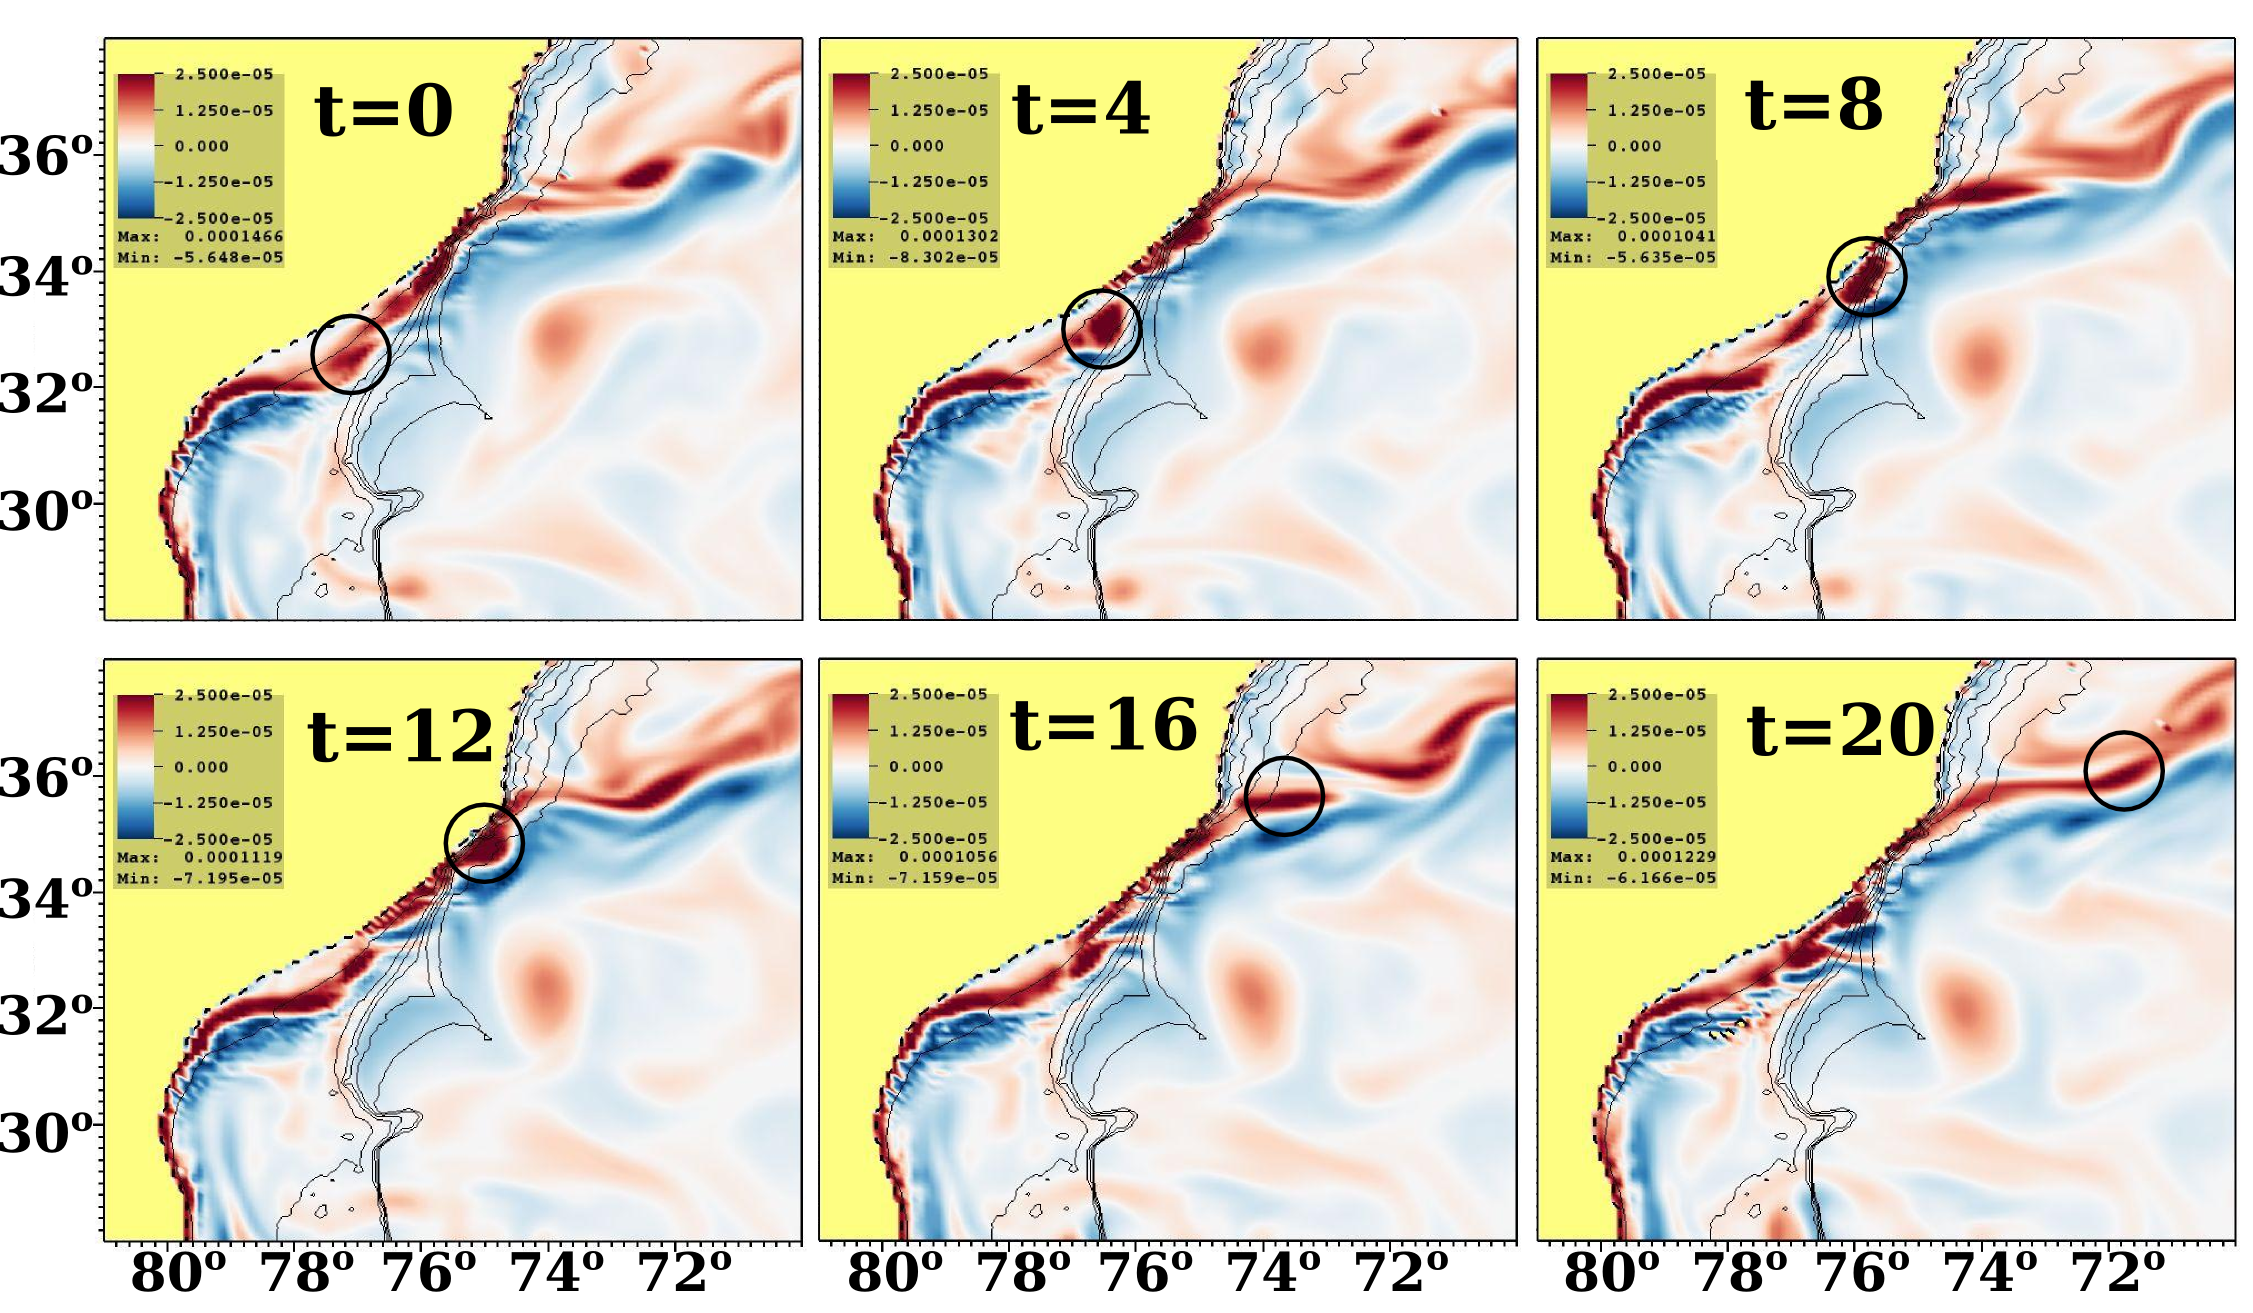
\includegraphics[scale=0.25]{figs/topographicwaves/vortices.png}
\caption{ The formation and subsequent progression of a cyclonic vortex is illustrated by looking at vorticity on a potential density surface ($\sigma_{500m} = 29.0 kg m^{-3}$). Each panel is a snapshot of the vorticity with four days of elapsed time between each. The cyclonic vortex that is shown (circled) is seen forming northeast of the Charleston Bump and subsequently travels northeastward torward Cape Hatteras where it is ``smeared-out.''}\label{fig:vortices}
\end{center}
\end{figure}

The theory in its current state is posed in a $1.5$ layer fluid and is not valid for flow speeds which equal the long baroclinic topographic wave speed given by
 \begin{equation}
 c = \frac{g\Delta \rho h_x}{\rho_0 f}.
 \end{equation}
 Thus, it has not been proven that flow separation is guaranteed for a continuously stratified (provided the criticality condition has been met). For a midlatitude coriolis parameter, topographic slope of $h_x \approx 1 \%$, and reduced gravity of $\frac{g\Delta \rho}{\rho0}\approx 10^{-2}m s^{-2}$, the long baroclinic topographic wave speed is $c \approx 1 m s^{-1}$. This speed is a typical scale for the Gulf Stream and suggests that there may be similar resonant interaction with higher order modes. Thus, in order to make further progress on explaining the separation problem, extending Stern's theory to include full stratification is necessary.  

In this document, a ``Linear-Long-Wave Theory" is outlined to demonstrate the demonstrate and explore topographic wave arrest. The linear framework presented provides an excellent starting point for future work in the study of large scale flow interactions with topography and can additionally be used towards forming a more complete story of the Gulf Stream separation and northward penetration. A numerical technique for the long wave equations, based in Spectral Element Methods, is outlined and validated following the presentation of the long topographic wave equations. The numerical technique is then applied to a continental shelf with length scales which correspond to the situation near Cape Hatteras. 

\section{Long Topographic Waves}
The equations of motion that are considered here are the Boussinesq, Hydrostatic primitive equations. These equations are argued to be valid for this problem as the lateral length scales for which we are concerned are far greater than the fluid depth. The problem we consider is that of a flow along a continental shelf which is modeled by the function
\begin{equation}
z=-h(x,y) = -\bar{h}(x) - \epsilon h'(x,y). \label{eq:generalBathy}
\end{equation} 
 The continental shelf is dominantly varying only in the $x$-direction and the degree of deviation from this is controlled by the small parameter $\epsilon$. As a final simplifying assumption, it is assumed that the along shelf length scales are far greater than the across shelf length scales, ie $L_y >> L_x$.   Along with the inviscid and adiabatic assumptions, the hydrostatic primitive equations reduce to 
  \begin{subequations}
  \begin{align}
  fv &= p_x \\
  v_t + uv_x + vv_y + wv_z + fu &= -p_y \\
  b_t + ub_x + v b_y + w b_z &= 0 \\
  p_z &= b \\
  w &= \vec{u} \cdot \nabla(\bar{h}(x) + \epsilon h'(x,y)), \text{ $z = -h(x,y)$}. \\
  w &= 0, \text{ $z =0$}
  \end{align} \label{eq:LongWaveEquations}
  \end{subequations}
The lateral velocity components are $u$ and $v$ and the vertical velocity component is $w$. The dynamic pressure (per unit mass) is denoted by $p$ is related to the buoyancy $b$ through hydrostatic balance. The buoyancy is defined as $b = -\frac{\rho' g}{\rho_0}$ where $\rho'$ is the density anomaly from a reference density $\rho_0$ and $g$ is the acceleration of gravity. The effects of planetary rotation are introduced via a coriolis acceleration with coriolis parameter $f$. On the topography and at the rigid fluid surface, no-normal-flow is enforced.

These equations are accurate to $\mathcal{O}\left( R\frac{L_x}{L_y} \right)$, where $R \equiv \frac{V}{fL_y}$ is the Rossby number. The assumptions used to arrive at \eqref{eq:LongWaveEquations} are essentially the same as those of \citet{Stern1998} except for the fact that, here, continuous stratification is accounted for. In addition to momentum conservation, equations \eqref{eq:LongWaveEquations} imply conservation of ``long-wave'' potential vorticity (PV) following fluid parcels where the PV is given by  
 \begin{equation}
 Q_{lw} = (v_x + f)b_z - v_z b_x \label{eq:pv}
\end{equation}    
   Expanding the ocean state variables (velocity, pressure, buoyancy, and PV) in orders of $\epsilon$ gives the $\mathcal{O}(1)$ equations as
   \begin{subequations}
   \begin{align}
   f \bar{v} &= \bar{p}_x \\
   \bar{p}_z &= b \\
   \bar{p} &= g \bar{\eta}, \hspace{4mm} \text{at }z=0\\
   \bar{b} &= \bar{b}(z) \\
   \bar{u} &= \bar{w} = 0.
   \end{align} \label{eq:orderONE}
   \end{subequations} 
 The overbar $\bar{\cdot}$ indicates the $\mathcal{O}(1)$ part of the expansion. The choice of $\bar{u} = \bar{w} = 0$ has been made, though a more general solution is possible. Additionaly, $\bar{v} = const.$ is chosen for simplicity and for other reasons that will soon become clear. The $\mathcal{O}(\epsilon)$ equations are
   \begin{subequations}
   \begin{align}
   v'_t + \bar{v} v'_y  + f u' &= -p'_y \\
   f v' &= p'_x\\
   b'_t + \bar{v} b'_y  + w' \bar{b}_z &= 0 \\
   p'_z &= b' \\
   \end{align}\label{eq:OrderEpsilon}
   \end{subequations}   
  with boundary conditions
     \begin{subequations}
   \begin{align}
   w'\bar{n}_z &= -u' \bar{n}_x - \bar{v}n'_y, \hspace{4mm} \text{at } z=-\bar{h}(x) \\
   w' &= 0 , \hspace{4mm} \text{at } z=0 \\
   p' &= 0, \hspace{4mm} \text{at } z=0.
   \end{align}
   \end{subequations}    
   The boundary normal, in general, is 
   \begin{equation}
   \hat{n} = \bar{n}_x \hat{x}  + \bar{n}_z \hat{z} + \epsilon \left( n'_x \hat{x}  + n'_y \hat{y} + n'_z \hat{z}\right)
   \end{equation}
   and can be determined from Equation \eqref{eq:generalBathy}.
   
   The PV equation for the hydrostatic primitive equations under the inviscid and adiabatic assumptions is
   \begin{equation}
   Q_t + uQ_x + vQ_y + wQ_z = 0 \label{eq:strat_pvconservation}
   \end{equation}
where the PV is given by equation \eqref{eq:pv}. We can split the PV into its two components plus a higher order correction,
  \begin{equation}
  Q =  f\bar{b}_z + \epsilon \left[  f b'_z +  v'_x \bar{b}_z \right] + \mathcal{O}(\epsilon^2) = \bar{Q} + \epsilon Q' + \mathcal{O}(\epsilon^2).
  \end{equation}
The $\mathcal{O}(\epsilon)$ PV equation is
  \begin{equation}
  Q'_t + \bar{v} Q'_y + w' \bar{Q}_z = 0 \label{eq:pvConservation}
  \end{equation}  
  where $\bar{Q}_x = 0$ identically by definition. The usual practice from here is to reduce Equation \eqref{eq:pvConservation} to an equation solely in terms of the pressure. To do this, the velocity and buoyancy corrections must be related to the pressure. Mass conservation and the $v$ momentum equation can be rearranged to yield a system for diagnosing the zonal and vertical velocities.
    \begin{subequations}
    \begin{align}
     u'  &= -\frac{1}{ f^2}\left[ \frac{D}{Dt}\frac{\partial}{\partial x}+ f \frac{\partial}{\partial y} \right]p' \\
   w'  &= -\frac{1}{N^2}\left[ \frac{D}{Dt}\frac{\partial }{\partial z}\right] p'
    \end{align}\label{eq:uAndw}
    \end{subequations}
where  $N^2 = \bar{b}_z$ is the squared buoyancy frequency and $\frac{D}{Dt} \equiv \frac{\partial}{\partial t} + \bar{v} \frac{\partial}{\partial y}$ denotes the derivative following the leading order flow.
    
  The potential vorticity anomaly can be expressed solely in terms of the dynamic pressure under the long wave approximation.
  \begin{equation}
  Q' = \mathcal{L}(p') =  \frac{N^2}{f^2} p'_{xx} + p'_{zz}  \label{eq:pvFromP}
  \end{equation}
  
It is assumed on the outset that the pressure can be decomposed as
\begin{equation}
p'(x,y,z,t) = \sum_{m=0}^{\infty} p_m \Psi_m(x,z) \phi_m(y,t).
\end{equation}
This reduces the PV equation to an equation in $(x,z)$ only
\begin{equation}
(\Psi_m)_{xx} + \left( \frac{f^2}{N^2} (\Psi_m)_z\right)_z = \nabla \cdot \vec{G}_m = 0. \label{eq:eqforpressure}
\end{equation}
It is convenient to define 
\begin{equation}
\vec{G}_m = (\Psi_m)_x \hat{x} + \frac{f^2}{N^2}(\Psi_m)_z \hat{z}.
\end{equation}
In hindsight, it is noted that this separation of variables is only possible for $\bar{v} = const.$. First, we will seek out the homogeneous solutions to this problem for which the the no-normal-flow boundary condition is
\begin{equation}
\sum_{m=0}^{\infty} p_m \left\lbrace \frac{D\phi_m}{Dt} \left( \frac{f^2}{N^2}(\Psi_m)_z\bar{n}_z  + (\Psi_m)_x \bar{n}_x \right) + f (\phi_m)_y \Psi_m\bar{n}_x \right\rbrace = 0, \label{eq:nonormalflow}
\end{equation}
In order for \eqref{eq:nonormalflow} to be true for any $p_m$, it must be the case that the factor inside the braces is zero for each $m$. Thus, Equation \eqref{eq:nonormalflow} implies that
\begin{subequations}
\begin{align}
(\phi_m)_t + (\bar{v} - c_m)(\phi_m)_y &= 0 \\
\vec{G}_m \cdot \hat{n} = -\frac{f\bar{n}_x}{c_m} \Psi_m
\end{align}
\end{subequations}
where $c_m$ is the speed of the $m^{th}$ topographic wave mode. Ultimately, the homogeneous system for the pressure reduces to
\begin{subequations}
\begin{align}
\nabla \cdot \vec{G}_m &= 0 \\
\vec{G}_m \cdot \hat{n} &= -\frac{ f\bar{n}_x \Psi_m }{c_m}, \text{ $z = -\bar{h}(x)$}\\
\vec{G}_m \cdot \hat{z} &= 0, \text{ $z = 0$ } \\
\Psi_m &\rightarrow 0, \text{ as $x\rightarrow \infty$} \\
(\phi_m)_t + (\bar{v} - c_m) (\phi_m)_y &= 0
\end{align}\label{eq:WaveProblem}
\end{subequations}
where $\hat{n} =  \bar{n}_x \hat{x} + \bar{n} \hat{z}$ is the outward pointing normal of the topography. Equations \eqref{eq:WaveProblem} form a system for determining the pressure field for topographic wave modes ($\Psi_m$) and the associated speeds ($c_m$).

We now proceed by demonstrating that the topographic waves travel in a direction such that (in the northern hemisphere) shallow bathymetry is to the right of the motion. Additionally, an orthogonality condition is derived which provides a method for including the effects of a steepening continental shelf. This last step illustrates how a steepening continental shelf can force topographic waves through a source of vortex tube stretching.

From the equation system \eqref{eq:WaveProblem}, a Rayleigh Quotient can be formed by multiplying (\ref{eq:WaveProblem}a) by $\Psi_m$, integrating and performing an integration by parts once. These steps yield 
\begin{equation}
c_m = -\frac{f \int_{shelf}\Psi_m^2 \bar{n}_x \hspace{1mm} dS }{\int ||\vec{G}_m||^2 \hspace{1mm} dV }. \label{eq:RayleighQuotient}
\end{equation}
As an example, take a continental shelf tht is described by $z(x) = -\alpha x$. For this simple case, the outward pointing boundary normal is proportional to
\begin{equation}
\vec{n} = -\alpha \hat{x} - \hat{z}
\end{equation}
so that $\bar{n}_x < 0 $ over the extent of the shelf. In the northern hemisphere, $f>0$. Thus, the Rayleigh Quotient given by Equation \eqref{eq:RayleighQuotient} indicates that $c_m > 0$ for every wave mode. In conjunction with Equation (\ref{eq:WaveProblem}e), if $\bar{v}=0$, the topographic wave modes travel in the $-y$ direction with the shallow water to the right of the wave propagation. This result is true in general for the northern hemisphere, namely that the waves  will travel with shallow water on the right. Because of this, only flows which travel with shallow water on their \textit{left} are capable of arresting topographic waves in the Northern Hemisphere. Currents which flow in the direction that is opposite the local topographic waves are called  \textit{retrograde}. Those that travel in the same direction as the local topographic waves are called \textit{prograde}. Now that we are aware of this general behavior, we now proceed to derive an orthogonality condition for this system.

In a similar manner as before, Equation (\ref{eq:WaveProblem}a) is multiplied by $\Psi_n$ and and integration by parts is performed once to give
\begin{equation}
\frac{f}{c_m}\int_{shelf}\Psi_m \Psi_n \bar{n}_x \hspace{1mm} dS = -\int (\Psi_m)_x (\Psi_n)_x + \frac{f^2}{N^2}(\Psi_m)_z (\Psi_n)_z \hspace{1mm} dV. \label{eq:orthoA}
\end{equation}
Similarly, it can be shown that
\begin{equation}
\frac{f}{c_n}\int_{shelf}\Psi_n \Psi_m \bar{n}_x \hspace{1mm} dS = -\int (\Psi_n)_x (\Psi_m)_x + \frac{f^2}{N^2}(\Psi_n)_z (\Psi_m)_z \hspace{1mm} dV. \label{eq:orthoB}
\end{equation}
Subtracting \eqref{eq:orthoB} from \eqref{eq:orthoA} gives 
\begin{equation}
f \left( \frac{1}{c_m}-\frac{1}{c_n} \right)\int_{shelf}\Psi_n \Psi_m \bar{n}_x \hspace{1mm} dS = 0
\end{equation} 
so that it must be the case that
\begin{equation}
\int_{shelf}\Psi_n \Psi_m \bar{n}_x \hspace{1mm} dS = \delta_{n,m} \int_{shelf} \Psi_m^2 \bar{n}_x \hspace{1mm} dS ,\label{eq:orthogonality}
\end{equation}
where $\delta_{m,n}$ denotes the Kronecker-Delta function. Equation \eqref{eq:orthogonality} is the orthogonality condition which will be used to solve the inhomogeneous problem.

The inhomogeneous solution solves the equation system \eqref{eq:WaveProblem} except that the no-normal flow boundary condition must be modified. Let the inhomogenous solution be expressed as
\begin{equation}
\tilde{p} = \sum_{m=0}^{\infty} \Psi_m(x,z)\phi_m(y,t)
\end{equation}
where the $\Psi_m$ are the homogenous topographic wave modes.  The no-normal flow boundary condition for the inhomogeneous case is 
\begin{equation}
\sum_{m=0}^{\infty} \left\lbrace \left( \frac{D\phi_m}{Dt} -c_m (\phi_m)_y \right) \left(\frac{ f }{c_m} \right) + F_m \right\rbrace\Psi_m \bar{n}_x = 0, \label{eq:nonormalflowINH}
\end{equation}
where the boundary forcing is expressed as a linear combination of the topographic wave modes
\begin{equation}
F(x,y,z) =  \frac{f^2 \bar{v} n'_y}{\bar{n}_x} = \sum_{m=0}^{\infty}F_m(y) \Psi_m(x,z).
\end{equation}
The orthogonality condition requires that each term in the sum expressed in Equation \eqref{eq:nonormalflowINH} must be zero independently so that
\begin{equation}
(\phi_m)_t + (\bar{v} - c_m) (\phi_m)_y = -\frac{c_m F_m}{f}.
\end{equation}
Thus, the inhomogeneous wave problem can be expressed
\begin{subequations}
\begin{align}
\nabla \cdot \vec{G}_m &= 0 \\
\vec{G}_m \cdot \hat{n} &= -\frac{ f\bar{n}_x \Psi_m }{c_m}, \text{ $z = -\bar{h}(x)$}\\
\vec{G}_m \cdot \hat{z} &= 0, \text{ $z = 0$ } \\
\Psi_m &\rightarrow 0, \text{ as $x\rightarrow \infty$} \\
(\phi_m)_t + (\bar{v} - c_m) (\phi_m)_y &= -\frac{c_m F_m}{f}\\
F_m &= \frac{\int_{shelf} f^2 \bar{v} n'_y\hspace{1mm} dS}{\int_{shelf} \Psi^2_m \bar{n}_x \hspace{1mm} dS}
\end{align}\label{eq:WaveProblemINH}
\end{subequations}
The key difference here is the inclusion of a fixed (in time) forcing term for the hyperbolic equation along the shelf. This forcing comes about by having a leading order flow which encounters the steepening (or broadening) of the continental shelf. By giving the bathymetry dependence in the $y$-direction, the leading order flow crosses isobaths and introduces a source of vortex tube stretching (or squashing). This drives the formation of topographic waves which then propagate at a speed of $\bar{v} - c_m$. This speed gives three classes of wave modes :
\begin{enumerate}
\item  The leading order flow is said to be \textit{supercritical} with respect to wave modes which satisfy $\bar{v} - c_m > 0$. Information from the steepening of the continental shelf travels in the direction of the leading order flow since the net speed is positive.
\item The leading order flow is said to be \textit{subcritical} with respect to wave modes which satisfy $\bar{v} - c_m < 0$. Information from the steepening of the continental shelf travels against the direction of the leading order flow since the net speed is negative.
\item \textit{Critical} topographic wave modes satisfy $c_m = \bar{v}$. These modes are stationary and, so long as $F_m \neq 0$, these modes exhibit resonance.
\end{enumerate}


\section{Relaxing the Long Wave Assumption}
If we relax the long wave assumption, then the $\mathcal{O}(\epsilon)$ equations are
   \begin{subequations}
   \begin{align}
   v'_t + \bar{v} v'_y + f u' &= -p'_y \\
   u'_t + \bar{v} u'_y - f v' &= -p'_x\\
   b'_t + \bar{v} b'_y  + w' \bar{b}_z &= 0 \\
   p'_z &= b' \\
   \end{align}\label{eq:OrderEpsilonShort}
   \end{subequations}   
  with boundary conditions
     \begin{subequations}
   \begin{align}
   w'\bar{n}_z &= -u' \bar{n}_x - \bar{v}n'_y, \hspace{4mm} \text{at } z=-\bar{h}(x) \\
   w' &= 0 , \hspace{4mm} \text{at } z=0 \\
   p' &= 0, \hspace{4mm} \text{at } z=0.
   \end{align}
   \end{subequations} 
The potential vorticity, to $\mathcal{O}(\epsilon^2)$ is
\begin{equation}
Q = f\bar{b}_z + \epsilon( \zeta \bar{b}_z + f p_{zz} ).
\end{equation}
The momentum equations imply that 
\begin{subequations}
\begin{align}
\left(\frac{D^2}{Dt^2} + f^2\right)u &= -( \frac{Dp_x}{Dt} + fp_y) \\
\left(\frac{D^2}{Dt^2} + f^2\right)v &= -( \frac{Dp_y}{Dt} - fp_x) 
\end{align}
\end{subequations}
so that we can relate the relative vorticity to the pressure through
\begin{equation}
\frac{D^2 \zeta}{Dt^2} = f (p_{xx} + p_{yy} )
\end{equation}
The equation governing the evolution of the potential vorticity becomes
\begin{equation}
\frac{D}{Dt}\left( p_{xx} + p_{yy} + \left(\frac{D^2}{Dt^2} + f^2 \right)\left(\frac{p_z}{N^2} \right)_z\right) =0
\end{equation}
The homogeneous no-normal flow condition can be written in terms of the pressure alone,
\begin{equation}
\left(\frac{D^2}{Dt^2} + f^2\right)\frac{p_z}{N^2}\bar{n}_z = ( \frac{Dp_x}{Dt} + fp_y) \bar{n}_x
\end{equation}
Separation of variables as before gives...
\pagebreak

\bibliography{bftirefs}
\bibliographystyle{plainnat}


\end{document}